The third question of the survey asks participants about their choice of presentational design patterns. In this question, MVVM, MVP, MVI, etc. design patterns were defined as presentational design patterns. The issue of why these design patterns are defined as presentational design patterns rather than architecture and criticisms on this subject can be found in section \ref{section:2.7}. When the results are  examined, we come across an exciting and also colourful picture. Below, in Fig \ref{fig:design_pattern} the participants' preferences for presentational design patterns can be seen.
\begin{figure}[ht!]
    \centering
    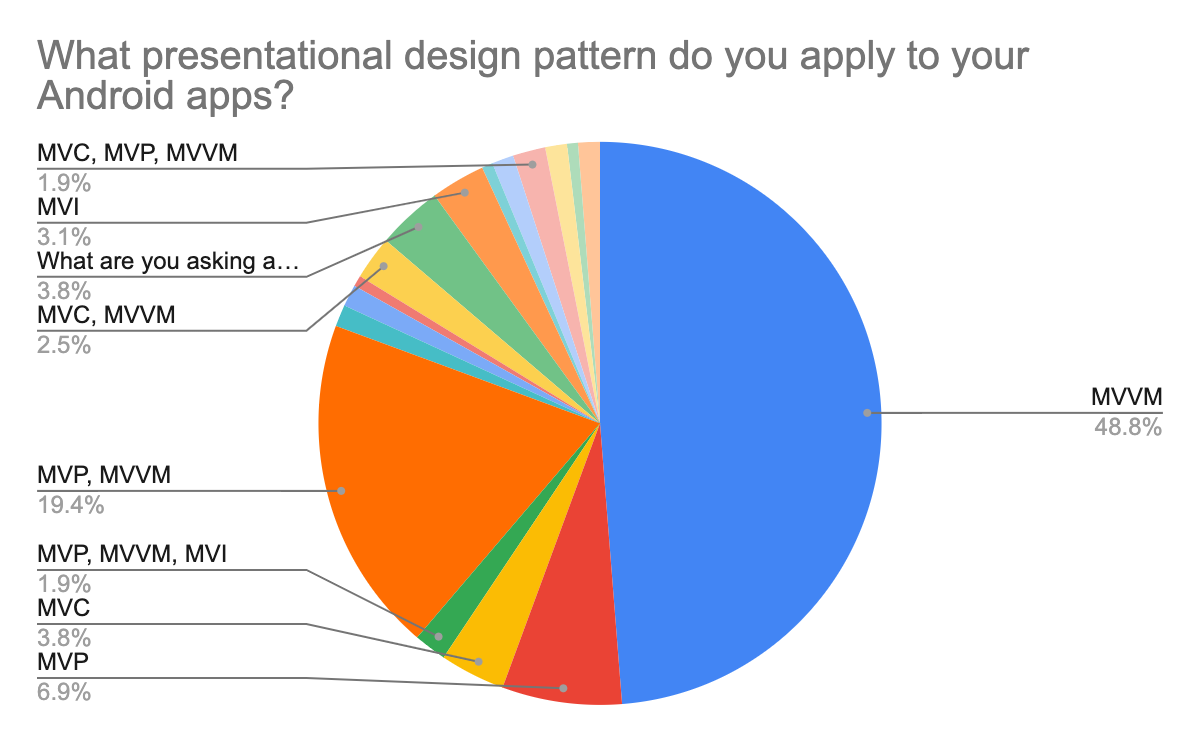
\includegraphics[scale=0.3]{figures/design_pattern.png}
    \caption{Presentational design patterns results}
    \label{fig:design_pattern}
\end{figure}
\FloatBarrier
The first notable conclusion is that almost half of the participants use the MVVM presentational design pattern. Besides, it is seen that another 25\% of the participants stated that they used this design pattern and different design patterns. In other words, a total of 3 quarters of the participants stated that they used the MVVM design pattern in some way or another. Android Architecture Components framework provides some out of box solutions for MVVM. We see that Android developers highly adopt it as of the first quarter of 2021. 

On the other hand, the chart presents us that design patterns such as MVP, MVC, MVI are also frequently used. When the participants' responses are sifted through, we see that design patterns such as MVP, MVC and MVI are generally preferred by some developers alongside the MVVM design pattern. These developers have more experience than those who have a single choice of design pattern. In other words,  it can be said that as the developer experience increases, the tendency of the developers to choose more than one design pattern also increases. In this case, it can be said that experienced Android developers make the presentational design pattern selection by considering which design pattern will fit the project size and content, rather than what is more popular. As another proof of this situation, it can be shown that developers with 0-3 years of experience have answered this question by selecting the MVVM option. In other words, it is possible to talk about the tendency of Android developers at the beginning of their career to choose popular or "hype" technologies. Another important detail is that 5 out of 6 participants that answered this question as "What are you asking about" had one year or less experience, proving that the knowledge of architecture and design pattern in software development correlates with experience. Lastly, concerning this question, it will be helpful to mention the participants’ tendency to choose design patterns such as MVC, MVP and MVI. Comparing the survey results with Figure 7, which is presented in section \ref{section:2.7} and cited from a study conducted a few years ago in Android architectures, we are faced with similar results despite minor differences. When we look at the comparison results, it is seen that MVVM and MVP were popular among the Android community a few years ago, but MVVM is more preferred today. As mentioned before, it can be said that since the MVVM design pattern started to be provided as an out of box solution by the Google Android team three years ago, this situation increased usage of the MVVM design pattern. In the survey, we also see that 18 of the participants declared that they used the MVC design pattern. Although the MVC design pattern is considered an outdated design pattern in the Android community, the existence of projects developed using this pattern, and considering the suitability of this pattern for small projects; it is understandable why the pattern is still in use. Finally, we see that the MVI design pattern was selected nine times in the last six months (out of 120 answers with a ratio of 0.075). However, it was selected only once (out of 40 answers with a ratio of 0.025) by the participants in the first six months in which the survey accepted answers. This fact is not surprising, given the MVI design pattern’s growing popularity during 2020 and 2021. It can be said that this population will increase even more in the upcoming period. As stated in section \ref{section:4.4.1}, Mooncascade's Android team prefers the MVVM presentational design pattern when developing Android applications. When the survey results (presented in detail above) and the company's choice are compared, it is seen that this choice coincides with the Android community’s current trends.

In the following question, users were asked whether they use the "Clean Architecture" structure. Detailed information about Clean Architecture has been given before in section \ref{section:4.4.2}. It is essential to mention why Clean Architecture was asked to the participants differently from the presentational design patterns. Clean Architecture allows the arrangement of an entire application in terms of architecture, unlike the presentational design patterns. The graphical breakdown of participant answers to this question is presented below in Fig \ref{fig:clean_arch}.
\begin{figure}[ht!]
    \centering
    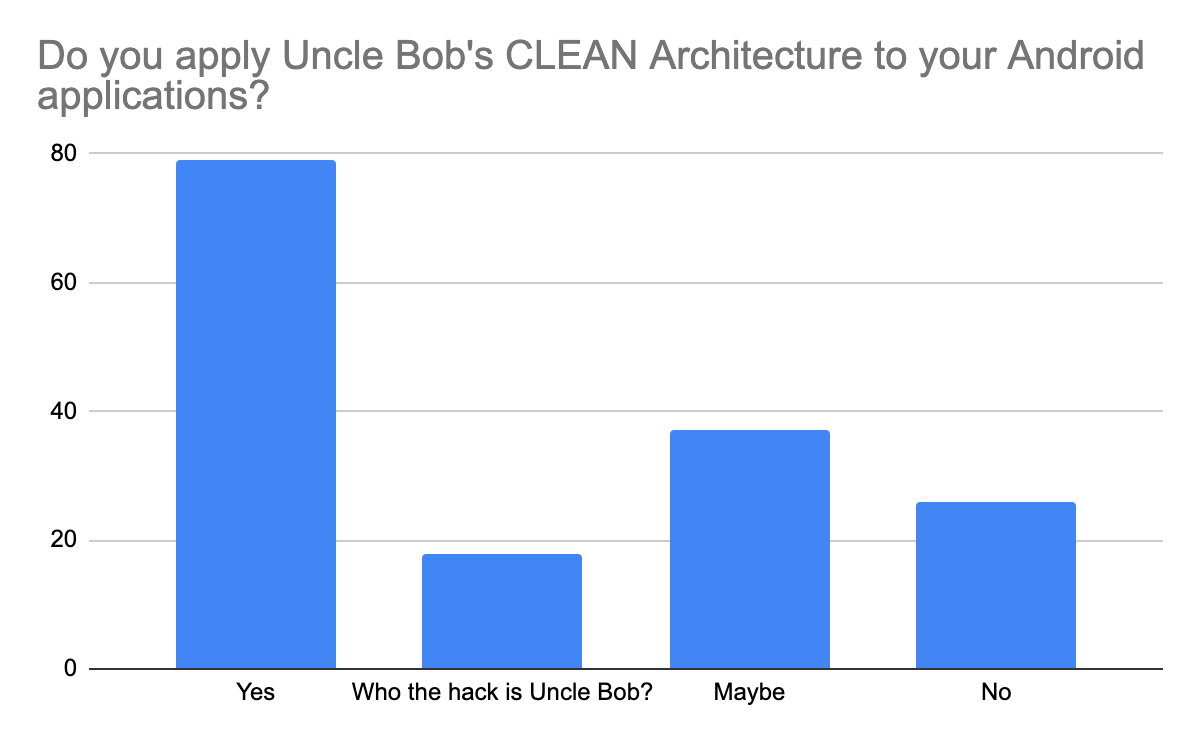
\includegraphics[scale=0.25]{figures/clean_arch.png}
    \caption{Clean Architecture usage results}
    \label{fig:clean_arch}
\end{figure}
\FloatBarrier

When examining the participatory tendencies to use Clean Architecture, it is seen that the majority of the participants adopt this architectural approach. The number of respondents who declared their use of this architectural pattern is almost more than the total of those who declared that they did not or could use it. Besides, 38 of 51 Android developers with five or more years of experience who participated in the survey declared that they use or can use this architectural pattern. Clean Architecture's details, pros and cons were previously shared, but it is widely used among developers, as seen from the survey results. As can be seen in Fig. \ref{fig:arch_patterns}, which is cited from a study on Android architecture carried out a few years ago. Considering the advantages of Clean Architecture, especially when developing large and complex Android applications, and the growing and complexity of Android applications, developers' choice of Clean Architecture makes much sense. Finally, it is possible to say that the Clean Architecture choice of the Mooncascade Android team coincides with the Android developer trends.